\documentclass{article}
\usepackage{tikz}
\usetikzlibrary{shapes.geometric, arrows.meta}

\begin{document}

\begin{figure}[h]
    \centering
    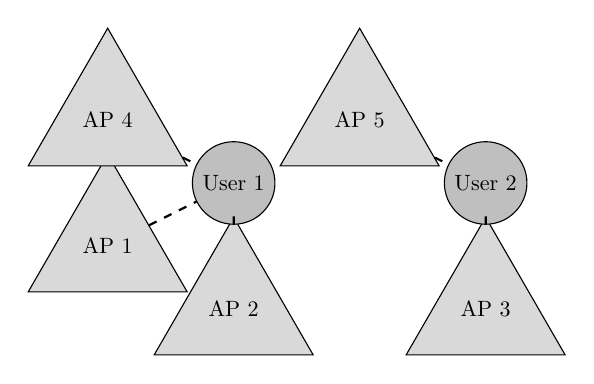
\begin{tikzpicture}[scale=0.8, transform shape]

        % Define styles for nodes
        \tikzset{
            ap/.style={draw, fill=gray!30, regular polygon, regular polygon sides=3, minimum size=1cm},
            user/.style={draw, fill=gray!50, circle, minimum size=0.7cm},
            line/.style={-Stealth, thick},
            dashed line/.style={dashed, thick}
        }

        % Draw APs
        \node[ap] (AP1) at (-2, 0) {AP 1};
        \node[ap] (AP2) at (0, -1) {AP 2};
        \node[ap] (AP3) at (4, -1) {AP 3};
        \node[ap] (AP4) at (-2, 2) {AP 4};
        \node[ap] (AP5) at (2, 2) {AP 5};

        % Draw users
        \node[user] (User1) at (0, 1) {User 1};
        \node[user] (User2) at (4, 1) {User 2};

        % Draw dashed lines for assignments
        \draw[dashed line] (AP1) -- (User1);
        \draw[dashed line] (AP2) -- (User1);
        \draw[dashed line] (AP3) -- (User2);
        \draw[dashed line] (AP4) -- (User1);
        \draw[dashed line] (AP5) -- (User2);

    \end{tikzpicture}
    \caption{\textbf{The mmWave CF network scenario in the downlink}, where dashed arrows indicate assignments between APs and users.}
    \label{fig:mmwave_cf_network}
\end{figure}

\end{document}